\documentclass[12pt, a4paper, oneside]{ctexart}
\usepackage{amsmath, amsthm, amssymb, bm, color, graphicx, geometry, mathrsfs,extarrows, braket, booktabs, array}
\usepackage[colorlinks,linkcolor=red,anchorcolor=blue,citecolor=blue,urlcolor=blue,menucolor=black]{hyperref}
%%%% 设置中文字体 %%%%
\setCJKmainfont{方正新书宋_GBK.ttf}[BoldFont=方正小标宋_GBK, ItalicFont=方正楷体_GBK]
%%%% 设置英文字体 %%%%
\setmainfont{Times New Roman}
\setsansfont{Calibri}
\setmonofont{Consolas}

\linespread{1.4}
%\geometry{left=2.54cm,right=2.54cm,top=3.18cm,bottom=3.18cm}
\geometry{left=1.84cm,right=1.84cm,top=2.18cm,bottom=2.18cm}
\newcounter{problem}  % 问题序号计数器
\newenvironment{problem}[1][]{\stepcounter{problem}\par\noindent\textbf{题目\arabic{problem}. #1}}{\smallskip\par}
\newenvironment{solution}[1][]{\par\noindent\textbf{#1解答. }}{\smallskip\par}  % 可带一个参数表示题号\begin{solution}{题号}
\newenvironment{note}{\par\noindent\textbf{注记. }}{\smallskip\par}

%%%% 图片相对路径 %%%%
\graphicspath{{figure/}} % 当前目录下的figure文件夹, {../figure/}则是父目录的figure文件夹
\setlength{\abovecaptionskip}{-0.2cm}  % 缩紧图片标题与图片之间的距离
\setlength{\belowcaptionskip}{0pt} 

\everymath{\displaystyle} % 默认全部行间公式
\DeclareMathOperator*\uplim{\overline{lim}} % 定义上极限 \uplim_{}
\DeclareMathOperator*\lowlim{\underline{lim}} % 定义下极限 \lowlim_{}
\DeclareMathOperator*{\argmax}{arg\,max}  % \argmin
\DeclareMathOperator*{\argmin}{arg\,min}  % \argmax
\let\leq=\leqslant % 将全部leq变为leqslant
\let\geq=\geqslant % geq同理

%%%% 一些宏定义 %%%%
\def\bd{\boldsymbol}        % 加粗(向量) boldsymbol
\def\disp{\displaystyle}    % 使用行间公式 displaystyle(默认)
\def\tsty{\textstyle}       % 使用行内公式 textstyle
\def\sign{\text{sign}}      % sign function
\def\wtd{\widetilde}        % 宽波浪线 widetilde
\def\R{\mathbb{R}}          % Real number
\def\N{\mathbb{N}}          % Natural number
\def\Z{\mathbb{Z}}          % Integer number
\def\Q{\mathbb{Q}}          % Rational number
\def\C{\mathbb{C}}          % Complex number
\def\N{\mathbb{N}}          % Natural number
\def\Z{\mathbb{Z}}          % Integer number
\def\E{\mathbb{E}}          % Exception
\def\var{\text{Var}}        % Variance
\def\bias{\text{bias}}      % bias
\def\d{\mathrm{d}}          % differential operator
\def\e{\mathrm{e}}          % Euler's number
\def\i{\mathrm{i}}          % imaginary number
\def\re{\mathrm{Re}}        % Real part
\def\im{\mathrm{Im}}        % Imaginary part
\def\res{\mathrm{Res}}      % Residue
\def\L{\mathcal{L}}         % Loss function
\def\wdh{\widehat}          % 宽帽子 widehat
\def\ol{\overline}          % 上横线 overline
\def\ul{\underline}         % 下横线 underline
\def\add{\vspace{1ex}}      % 增加行间距
\def\del{\vspace{-1.5ex}}   % 减少行间距

%%%% 定理类环境的定义 %%%%
\newtheorem{theorem}{定理}

%%%% 基本信息 %%%%
\newcommand{\RQ}{\today} % 日期
\newcommand{\km}{数理统计} % 科目
\newcommand{\bj}{强基数学002} % 班级
\newcommand{\xm}{吴天阳} % 姓名
\newcommand{\xh}{2204210460} % 学号
\newcommand{\id}{50} % 序号

\begin{document}

%\pagestyle{empty}
\pagestyle{plain}
\vspace*{-15ex}
\centerline{\begin{tabular}{*6{c}}
    \parbox[t]{0.25\linewidth}{\begin{center}\textbf{日期}\\ \large \textcolor{blue}{\RQ}\end{center}} 
    & \parbox[t]{0.2\linewidth}{\begin{center}\textbf{科目}\\ \large \textcolor{blue}{\km}\end{center}}
    & \parbox[t]{0.2\linewidth}{\begin{center}\textbf{班级}\\ \large \textcolor{blue}{\bj}\end{center}}
    & \parbox[t]{0.1\linewidth}{\begin{center}\textbf{姓名}\\ \large \textcolor{blue}{\xm}\end{center}}
    & \parbox[t]{0.15\linewidth}{\begin{center}\textbf{学号}\\ \large \textcolor{blue}{\xh}\end{center}}
    & \parbox[t]{0.1\linewidth}{\begin{center}\textbf{序号}\\ \large \textcolor{blue}{\id}\end{center}}
     \\ \hline
\end{tabular}}
\begin{center}
    \zihao{3}\textbf{第五次作业}
\end{center}\vspace{-0.2cm}
% 正文部分
\begin{problem}[(44)]
    令$X_1,\cdots,X_n$是来自$f(x;\theta)=\e^{-(x-\theta)}I_{[\theta,\infty)}(x),\ (\theta\in \R^1)$的随机样本.

    (a). 求解一个充分统计量.

    (b). 求出$\theta$的MLE.

    (c). 求出$\theta$的矩估计.

    (d). 求解一个完备充分统计量.

    (e). 求解$\theta$的UMVUE.

    (f). 求出关于$\theta$的Pitman估计量.

    (g). 使用先验分布$g(\theta) = \e^{-\theta}I_{(0,\infty)}(\theta)$,求出$\theta$的后验Bayes估计量.
\end{problem}
\begin{solution}
    (a). 由于$f(x;\theta) = 1\cdot I_{[\theta,\infty)}(x)\exp\left\{\theta-x\right\}$,令$a(\theta) = 1,\ b(x) = I_{[\theta,\infty)}(x),\ c(\theta)=\theta,\ d(x) = -x$,于是$-\sum_{i=1}^nX_i$是完备充分统计量.

    (b). 由于$\L(\theta) = \prod_{i=1}^nf(x_i;\theta) = \prod_{i=1}^n\e^{-(x_i-\theta)}I_{[\theta,\infty)}(x_i) = \exp\left\{-\sum_{i=1}^nx_i+n\theta\right\}I_{(-\infty,y_1]}(\theta)$,其中$Y_1 = \min\{X_1,\cdots,X_n\}$,则MLE为$\hat{\theta}=Y_1$.\add

    (c). $\E(\bar{X}) = \E(X) = \int_{\theta}^\infty x\e^{-(x-\theta)}\,\d x = \int_{0}^\infty(x+\theta)\e^{-x}\,\d x = \frac{\Gamma(2)}{1^2}+\theta = 1+\theta$,于是$\theta$的矩估计为$\tilde{\theta}=\bar{X}-1$.

    (d). 由(a)可知,$-\sum_{i=1}^nX_i$是完备充分统计量.

    (e). 由于$\bar{X}-1$是关于$-\sum_{i=1}^nX_i$的统计量且是$\theta$的无偏估计,于是$\bar{X}-1$是$\theta$的UMVUE.

    (f).

    (g). 由于$\L(\theta) = \e^{n\theta-\sum_{i=1}^nx_i}I_{(-\infty, y_1]}(\theta)\propto \e^{n\theta}I_{(-\infty,y_1]}(\theta)$且$f(\theta|x_1,\cdots, x_n) = \int L(\theta)g(\theta)\,\d\theta = \int_0^{y_1}\e^{(n-1)\theta}\,\d\theta = \frac{\e^{(n-1)y_1}-1}{n-1},\ (y_1>0)$.则
    \begin{equation*}
        f(\theta|x_1,\cdots,x_n) = \frac{\L(\theta)g(\theta)}{\int L(\theta)g(\theta)\,\d\theta} = \frac{n-1}{\e^{(n-1)y_1}-1}\e^{(n-1)\theta}I_{(0,y_1]}(\theta).
    \end{equation*}
    于是
    \begin{align*}
        \E\left[\theta|x_1,\cdots,x_n\right] =&\ \int_0^{y_1}\theta\frac{n-1}{\e^{(n-1)y_1}-1}\e^{(n-1)\theta}\,\d\theta = \frac{n-1}{\e^{(n-1)y_1}-1}\int_0^{y_1}\theta\e^{-(1-n)\theta}\,\d\theta\\
        =&\ \frac{n-1}{\e^{(n-1)y_1}-1}\cdot\frac{\Gamma(2)}{(1-n)^2} = \frac{1}{(n-1)(\e^{(n-1)y_1}-1)}
    \end{align*}
    则$\theta$的后验Bayes估计量为$\frac{1}{(n-1)(\e^{(n-1)y_1}-1)}$.
\end{solution}
\begin{problem}[(47)]
    令$X_1,\cdots,X_n$是来自离散分布$f(x;\theta) = \binom{2}{x}\theta^x(1-\theta)^{2-x}I_{\{0,1,2\}}(x),\ (\theta > 0)$的随机变量.

    (a). 是否存在一维的充分统计量,若存在,是否完备?

    (b). 求解$\theta^2 = P(X_1=2)$的MLE,并判断是否是无偏的.

    (c). 求解一个关于$\theta$的无偏统计量,且满足C-R下界. 若不存在,证明之.

    (d). 求解一个$\theta^2$的UMVUE.

    (e). 利用平方误差损失函数求解$\theta^2$关于先验分布为Beta分布的Bayes估计. Beta分布为$g(\theta) = \frac{1}{B(a,b)}\theta^{a-1}(1-\theta)^{b-1}I_{(0,1)}(\theta)$.

    (f). 使用平方误差损失函数,求解$\theta$的最大估计.

    (g). 求解$\theta^2$均方误差的一致估计.
\end{problem}
\begin{solution}
    (a). 由于
    \begin{equation*}
        f(x;\theta) = \exp\{2\log(1-\theta)\}\binom{2}{x}I_{\{0,1,2\}}(x)\exp\left\{x\log\frac{\theta}{1-\theta}\right\}   
    \end{equation*}
    令$a(\theta) = \exp\{2\log(1-\theta)\},\ b(x) = \binom{2}{x}I_{\{0,1,2\}}(x),\ c(\theta) = \log\frac{\theta}{1-\theta},\ d(x) = x$. 则$\sum_{i=1}^nX_i$是完备充分统计量.

    (b). 
\end{solution}

% 下面给一些功能的写法
\iffalse
% 图片模板
\centerline{
    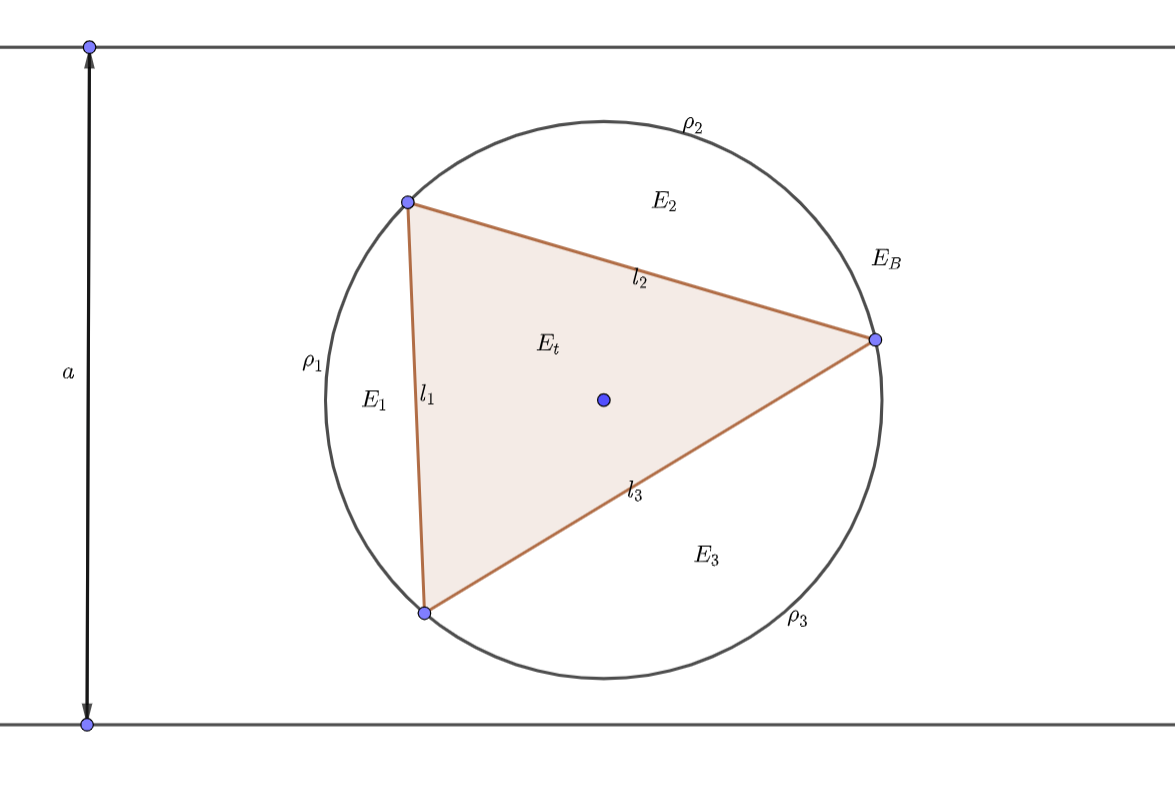
\includegraphics[width=0.8\textwidth]{figure.png}
}
% 表格模板
\renewcommand\arraystretch{0.8} % 设置表格高度为原来的0.8倍
\begin{table}[!htbp] % table标准
    \centering % 表格居中
    \begin{tabular}{p{1cm}<{\centering}p{1cm}<{\centering}p{3cm}<{\centering}p{5cm}<{\centering}} % 设置表格宽度
    %\begin{tabular}{cccc}
        \toprule
        $x_i$ & $f[x_1]$ & $f[x_i,x_{i+1}]$ & $f[x_i,x_{i+1},x_{i+2}]$ \\
        \midrule
        $x_0$ & $f(x_0)$ &                  &                          \\
        $x_0$ & $f(x_0)$ & $f'(x_0)$        &                          \\
        $x_0$ & $f(x_1)$ & $\frac{f(x_1)-f(x_0)}{x_1-x_0}$ & $\frac{f(x_1)-f(x_0)}{(x_1-x_0)^2}-\frac{f'(x_0)}{x_1-x_0}$\\
        \bottomrule
    \end{tabular}
\end{table}

\def\Log{\text{Log}} % 一个简单的宏定义
$\Log$ % 调用方法
\fi

\end{document}